\subsection{Diagrama de Classes}

O sistema foi projetado seguindo uma hierarquia de herança clara para o acervo bibliográfico. A classe abstrata \texttt{ItemAcervo} define o contrato comum para todos os itens do acervo, sendo estendida pelas classes concretas \texttt{LivroFisico} e \texttt{EBook}.

\begin{figure}[htbp]
	\centering
	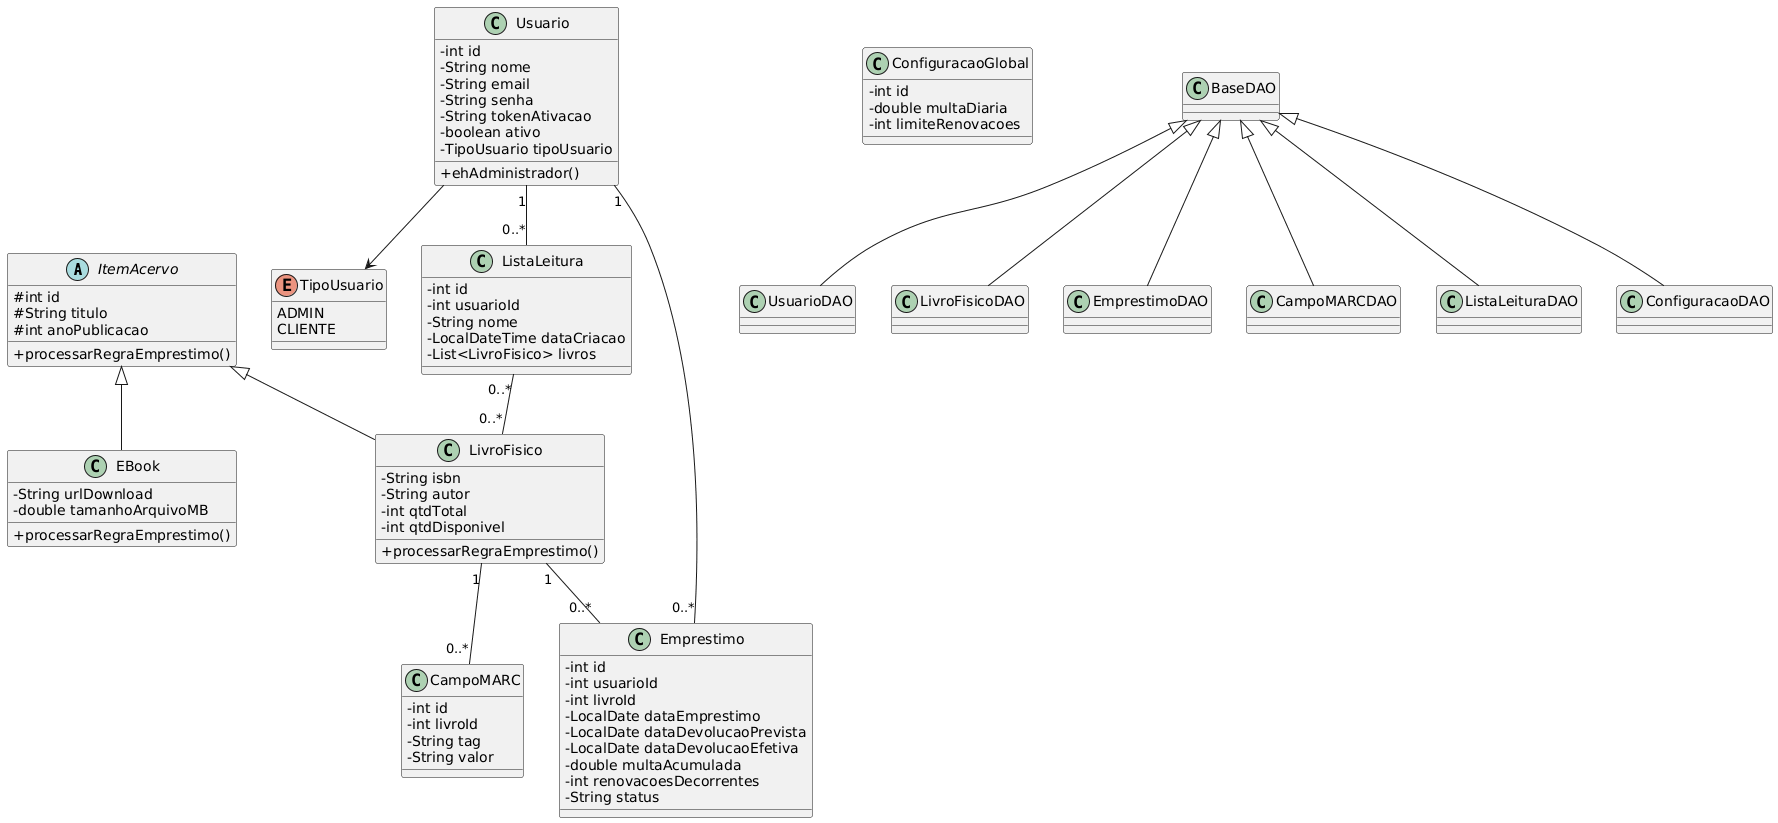
\includegraphics[width=\textwidth,height=0.72\textheight,keepaspectratio]{../imagens/1-class_diagram.png}
	\caption{Diagrama de Classes do sistema Biblioteca MARC21}
	\label{fig:diagrama-classes}
\end{figure}

As principais relações de herança e associação são:

\begin{itemize}
	\item \textbf{\texttt{ItemAcervo} (Abstrata)} $\leftarrow$ \texttt{LivroFisico}: Representa obras físicas do acervo com controle de quantidade disponível em estoque.
	\item \textbf{\texttt{ItemAcervo} (Abstrata)} $\leftarrow$ \texttt{EBook}: Representa livros digitais com URL de acesso e sem restrição de quantidade.
	\item \textbf{\texttt{BaseDAO} (Abstrata)} $\leftarrow$ Todos os DAOs: Centraliza a lógica de obtenção de conexão JDBC.
	\item \textbf{\texttt{Emprestimo}} associa \texttt{Usuario} e \texttt{LivroFisico}: Representa a solicitação e, após aprovação administrativa, o contrato de retirada física.
\end{itemize}

\subsection{Arquitetura de Fluxo de Dados}

O fluxo de execução das requisições assíncronas (AJAX) segue de forma padronizada o seguinte caminho:

\begin{center}
	\texttt{Navegador} $\xrightarrow{\text{HTTP Request}}$ \texttt{AutenticacaoFilter} $\rightarrow$ \texttt{XServlet} $\rightarrow$ \texttt{XServletDAO} $\rightarrow$ \texttt{MySQL} \\[0.3cm]
	\texttt{MySQL} $\xrightarrow{\text{ResultSet}}$ \texttt{XServletDAO} $\rightarrow$ \texttt{Gson.toJson()} $\xrightarrow{\text{JSON}}$ \texttt{jQuery/AJAX} $\rightarrow$ \texttt{DOM}
\end{center}

\subsection{Diagrama Entidade-Relacionamento}

O modelo relacional do banco de dados organiza os cadastros principais e as relações operacionais de empréstimo, metadados MARC21 e listas de leitura.

\begin{figure}[htbp]
	\centering
	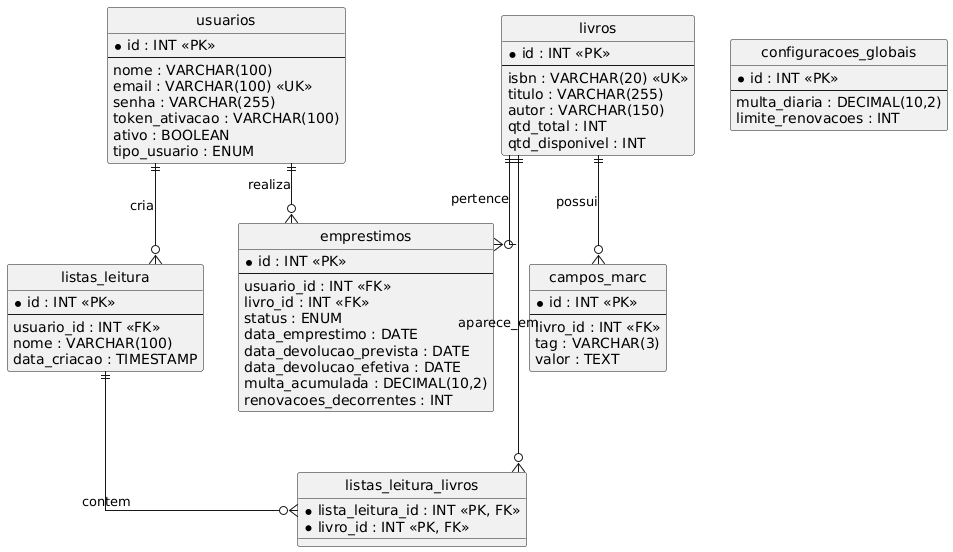
\includegraphics[width=\textwidth,height=0.72\textheight,keepaspectratio]{../imagens/2-entity_diagram.png}
	\caption{Diagrama Entidade-Relacionamento do banco de dados}
	\label{fig:diagrama-er}
\end{figure}

\subsection{Diagrama de Caso de Uso}

\begin{figure}[htbp]
	\centering
	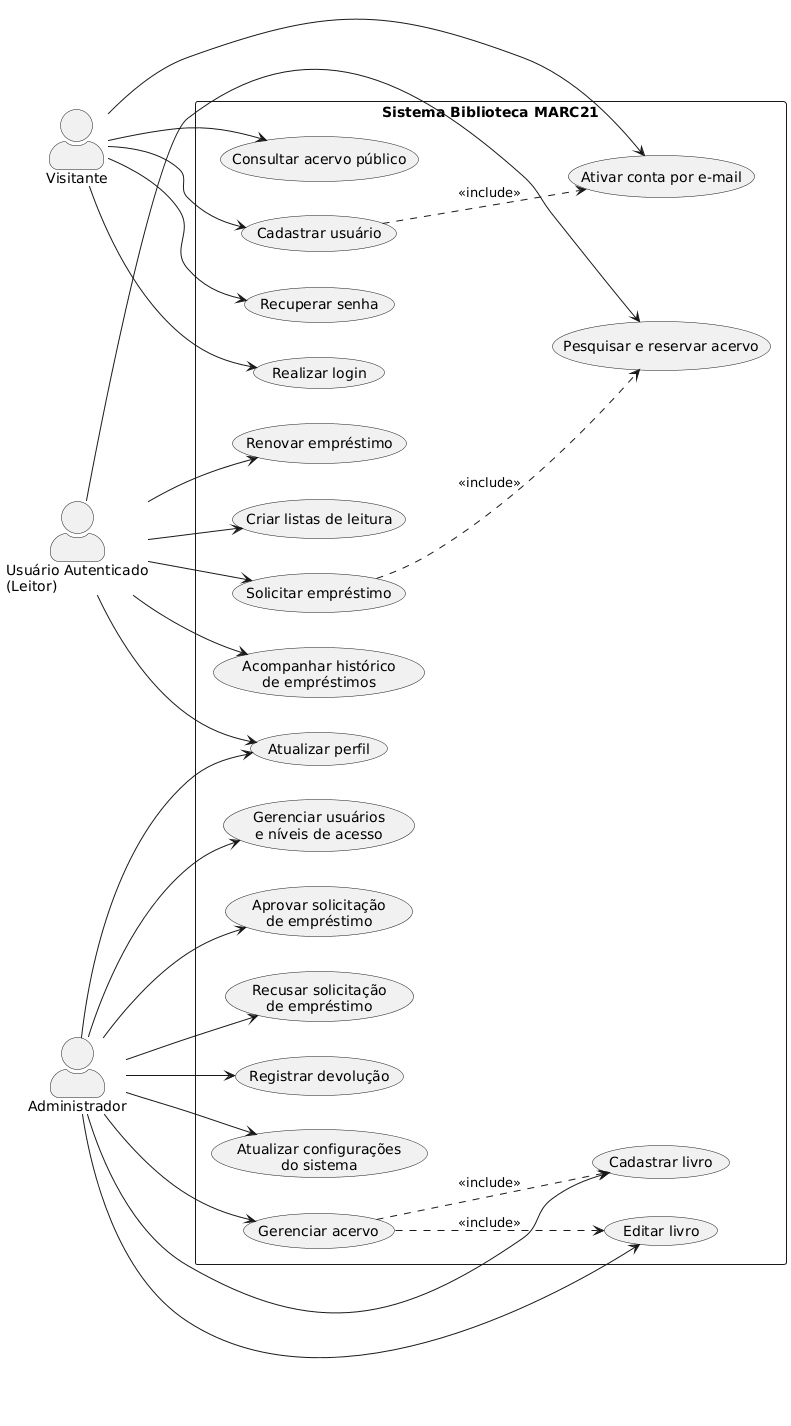
\includegraphics[width=\textwidth,height=0.72\textheight,keepaspectratio]{../imagens/3-use_case_diagram.png}
	\caption{Diagrama de Caso de Uso}
	\label{fig:diagrama-caso-uso}
\end{figure}

\subsection{Diagrama de Sequência: Solicitação e Aprovação de Empréstimo}

\begin{figure}[htbp]
	\centering
	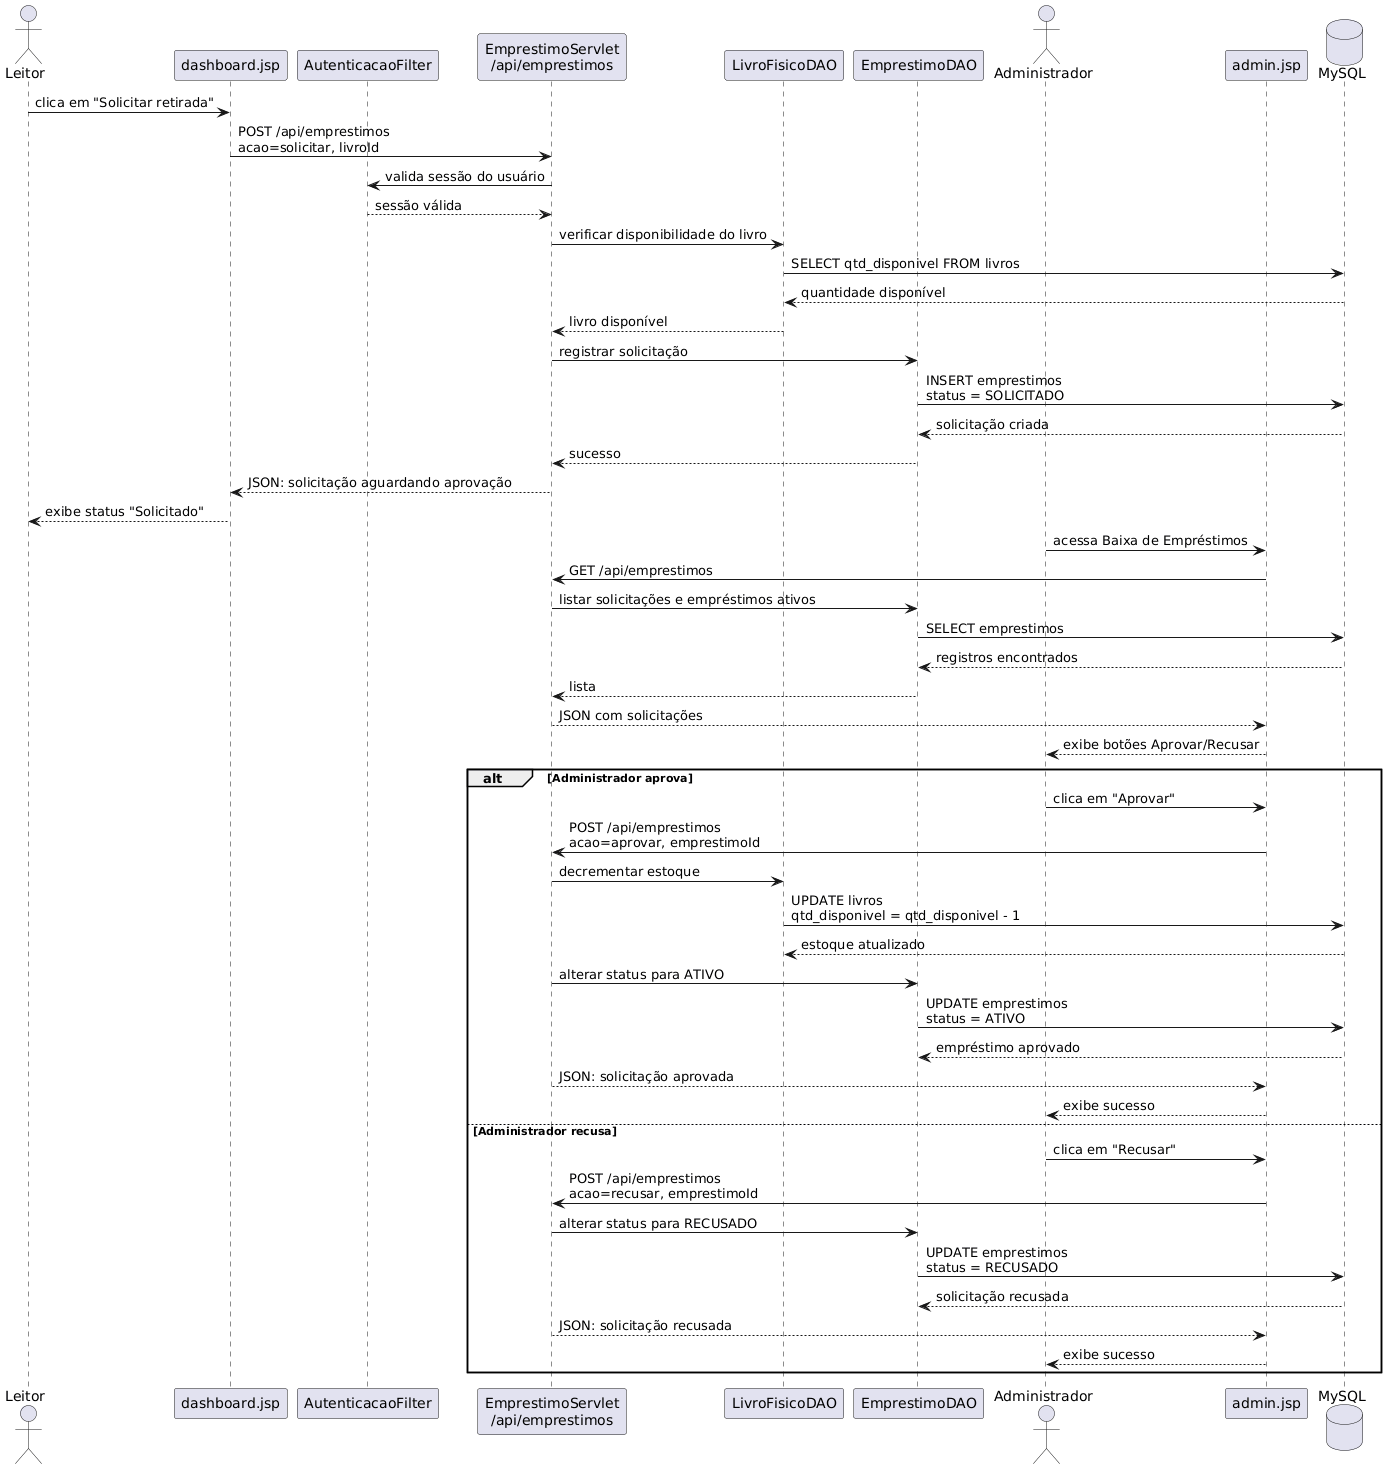
\includegraphics[width=\textwidth,height=0.72\textheight,keepaspectratio]{../imagens/4-sequence_diagram.png}
	\caption{Diagrama de Sequência: solicitação e aprovação de empréstimo}
	\label{fig:diagrama-sequencia-emprestimo}
\end{figure}
